
\frame
{
\frametitle{\citetitle{MarcoNuno_CongArbIng_2003_12_00}}
\begin{columns}
  \column {0.5\textwidth}  
En ese artículo se reportan dos arquitecturas hardware:
\begin{itemize}
\item Estimación de la pirámide de imágenes
\item Calcular la correlación entre dos imágenes
\end{itemize}
Tres aplicaciones:
\begin{itemize}
\item Seguimiento.
\item Estabilización.
\item Generación de mosaicos.
\end{itemize}
  \column {0.5\textwidth}  
  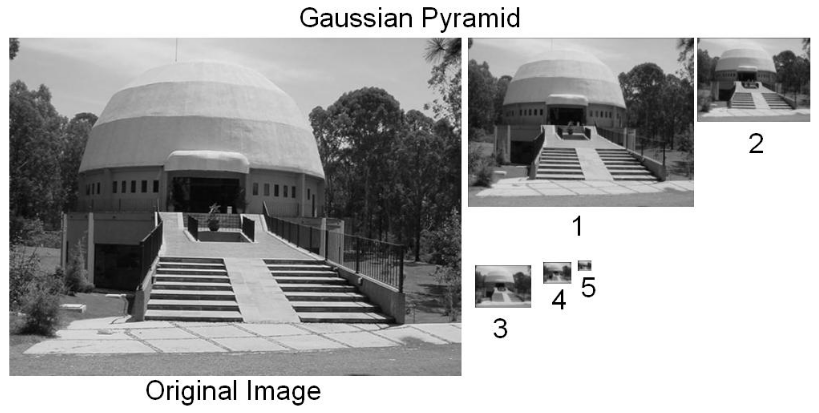
\includegraphics[width=0.9\textwidth]{Figs/Piramide}
  \end{columns}
\footnotetext[1]{\fullcite{MarcoNuno_CongArbIng_2003_12_00}}
}

\frame{
\frametitle{Seguimiento, Estabilización y Mosaicos}
\begin{columns}
    \column {0.5\textwidth}
    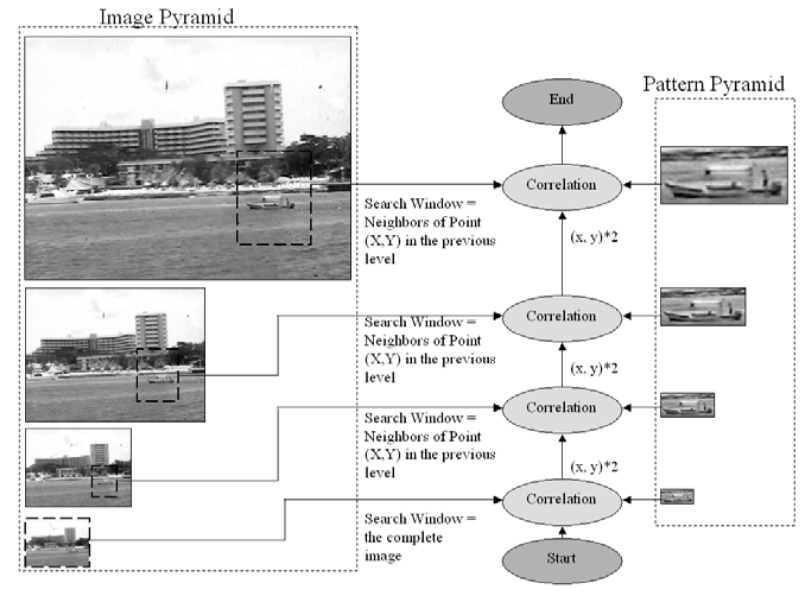
\includegraphics[width=0.9\textwidth]{Figs/Piramide_Correlacion}
    \column {0.5\textwidth}    
        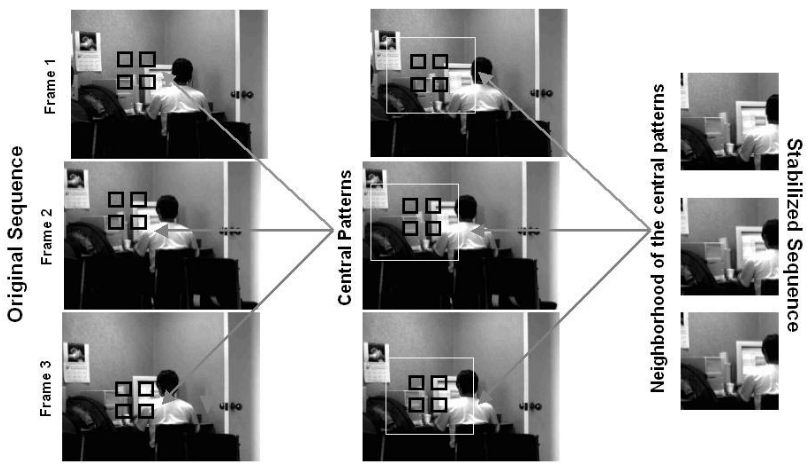
\includegraphics[width=0.8\textwidth]{Figs/Piramide_Estabilizacion}\\
        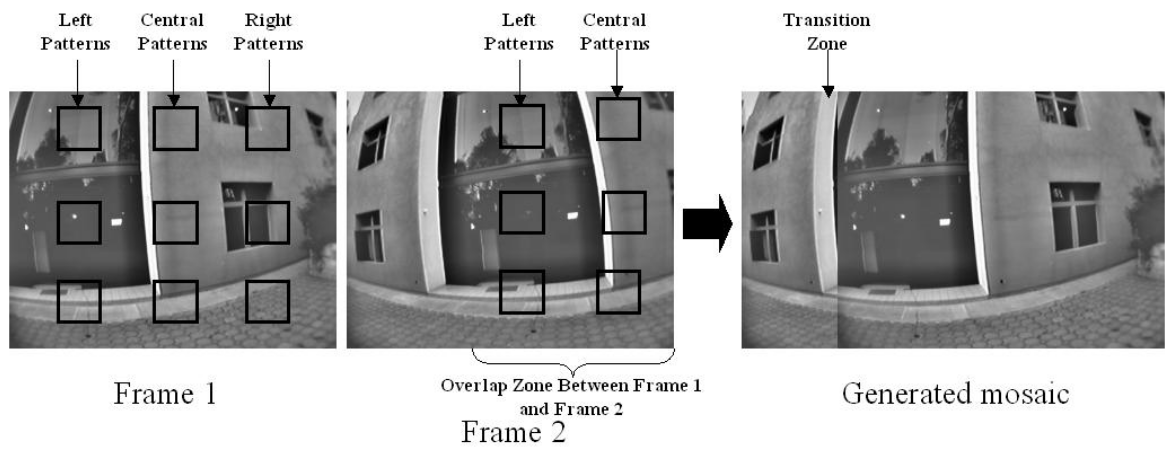
\includegraphics[width=0.98\textwidth]{Figs/Piramide_Mosaicos}
      
\end{columns}    
}

\frame{
\frametitle{Resultados}
    \begin{columns}
        \column {0.5\textwidth}
            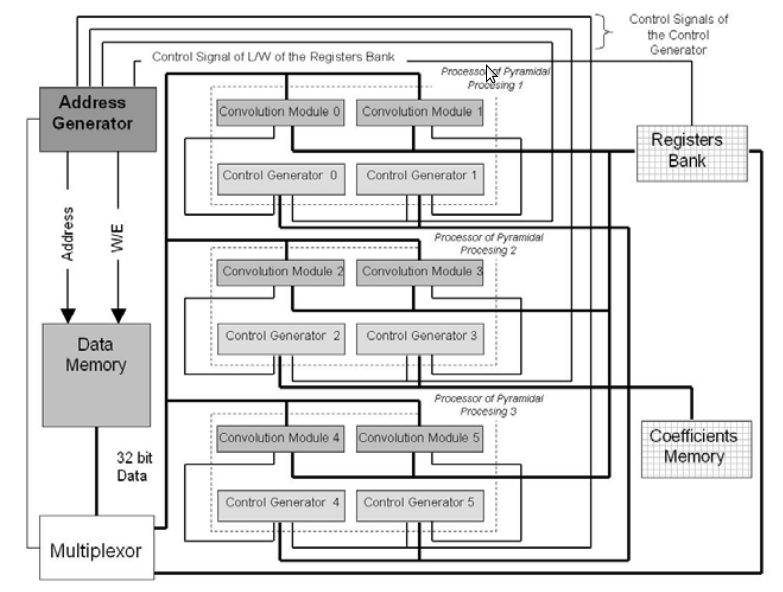
\includegraphics[width=0.8\textwidth]{Figs/Piramide_Arquitectura1}
        \column {0.5\textwidth}    
            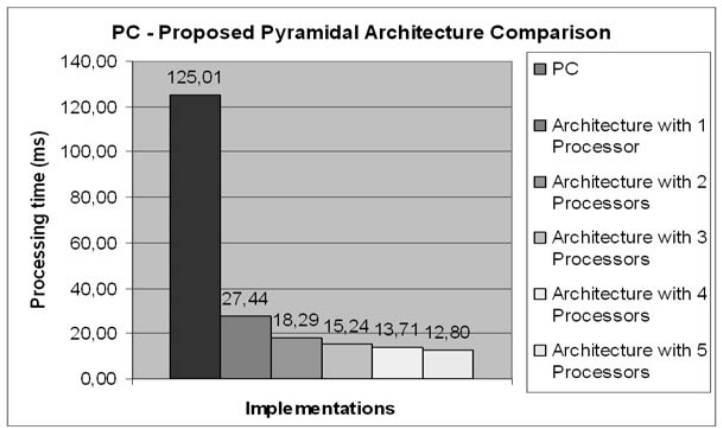
\includegraphics[width=0.9\textwidth]{Figs/Piramide_GraficaComparacion}
    \end{columns}    
}

